\documentclass[10pt,landscape]{article}
\usepackage{multicol}
\usepackage{calc}
\usepackage{ifthen}
\usepackage[portrait]{geometry}
\usepackage{hyperref}
\usepackage{blindtext}
\usepackage{amssymb,amsmath}
\usepackage{siunitx}
\usepackage{tikz}
\usetikzlibrary{decorations.pathmorphing}
\usepackage{makecell}
\usepackage[none]{hyphenat}
\usepackage{wrapfig}
\usepackage{float}

\tikzset{snake it/.style={decorate, decoration=snake}}

% Additional Units
\DeclareSIUnit\curie{Ci}
\DeclareSIUnit\number{\#}
\DeclareSIUnit\clight{\ensuremath{c}}
\DeclareSIUnit\rad{rad}
\DeclareSIUnit\rem{rem}
\DeclareSIUnit\roentgen{R}

% Math Operators
\DeclareMathOperator{\atan}{atan}

% This sets page margins to .5 inch if using letter paper, and to 1cm
% if using A4 paper. (This probably isn't strictly necessary.)
% If using another size paper, use default 1cm margins.
\ifthenelse{\lengthtest { \paperwidth = 11in}}
	{ \geometry{top=.5in,left=.5in,right=.5in,bottom=.5in} }
	{\ifthenelse{ \lengthtest{ \paperwidth = 297mm}}
		{\geometry{top=1cm,left=1cm,right=1cm,bottom=1cm} }
		{\geometry{top=1cm,left=1cm,right=1cm,bottom=1cm} }
	}

% Turn off header and footer
\pagestyle{empty}

% Redefine section commands to use less space
\makeatletter
\renewcommand{\section}{\@startsection{section}{1}{0mm}%
                                {-1ex plus -.5ex minus -.2ex}%
                                {0.5ex plus .2ex}%x
                                {\normalfont\large\bfseries}}
\renewcommand{\subsection}{\@startsection{subsection}{2}{0mm}%
                                {-1explus -.5ex minus -.2ex}%
                                {0.5ex plus .2ex}%
                                {\normalfont\normalsize\bfseries}}
\renewcommand{\subsubsection}{\@startsection{subsubsection}{3}{0mm}%
                                {-1ex plus -.5ex minus -.2ex}%
                                {1ex plus .2ex}%
                                {\normalfont\small\bfseries}}
\makeatother

% Define BibTeX command
\def\BibTeX{{\rm B\kern-.05em{\sc i\kern-.025em b}\kern-.08em
    T\kern-.1667em\lower.7ex\hbox{E}\kern-.125emX}}

% Don't print section numbers
\setcounter{secnumdepth}{0}

\setlength{\parindent}{0pt}
\setlength{\parskip}{0pt plus 0.5ex}

\begin{document}

%\raggedright
\footnotesize
\begin{multicols*}{3}

% multicol parameters
% These lengths are set only within the two main columns
\setlength{\premulticols}{1pt}
\setlength{\postmulticols}{1pt}
\setlength{\multicolsep}{1pt}
\setlength{\columnsep}{2pt}

\begin{center}
     \Large{\textbf{Nuclear Engineering}} \\
\end{center}

\section{Units \& Conversions}
\begin{align*}
\hbar & = \SI{1.05457e-34}{\joule\second} \\
c & = \SI{2.997925e8}{\meter\per\second} \\
h c & = \SI{1.240e-6}{\electronvolt\meter} \\
k_0 & = \SI{8.99e9}{\newton\square\meter\per\square\coulomb} \\
N_0 & = \SI{6.0221e23}{\per\mole} \\
\SI{1}{\mega\electronvolt} & = \SI{1.60218e-27}{\joule} \\
\SI[per-mode=symbol]{1}{\mega\eV\per\clight\squared} & = \SI{1.78266e-30}{\kilo\gram} \\
1~\text{AMU} & = \SI{1.66054e-27}{\kilo\gram} \\
\quad & = \SI[per-mode=symbol]{931.494}{\mega\eV\per\clight\squared} \\
\text{M}_\text{Proton} & = \SI[per-mode=symbol]{928.272}{\mega\eV\per\clight\squared} \\
\text{M}_\text{Neutron} & = \SI[per-mode=symbol]{939.565}{\mega\eV\per\clight\squared} \\
\text{M}_\text{Electron} & = \SI[per-mode=symbol]{0.511}{\mega\eV\per\clight\squared} \\
\SI{1}{\barn} & = \SI{1e-24}{\cm} \\
\SI{1}{\curie} & = \SI{3.7e10}{\becquerel} \\
\SI{1}{\coulomb} & = \SI{1.602e-19}{\elementarycharge} \\
\SI{1}{\roentgen} & = \SI{2.58e-4}{\coulomb\per\kilo\gram}
\end{align*}
\SI{1}{\curie} is roughly the activity of \SI{1}{\gram} of Ra\textsuperscript{226}
\section{Terms \& Basic Facts}
\begin{equation*}
X^A_Z \quad \!
\begin{aligned}
    \text{X} &= \text{Chemical Symbol} \\
    \text{A} &= \text{Mass Number (\# nucleons)} \\
    \text{Z} &= \text{Atomic Number (\# protons)} \\
\end{aligned}
\end{equation*}

dN particles incident on sphere with $\sigma$ area dA
\begin{align*}
&\text{Fluence} & \Phi &= \frac{dN}{dA} ~ [\si{\per\square\meter}] \\
&\text{Fluence Rate, Flux} & \dot{\Phi} &= \frac{d\Phi}{dt} ~ [\si{\per\square\meter\per\second}]
\end{align*}
For a specified volume, \\
$R_\text{in}, R_\text{out}$ are radiant K.E. incident and emerging \\
$Q$ is a change in rest mass of nuclei or particle
\begin{align*}
&\text{Energy Imparted} & \epsilon &= R_\text{in} - R_\text{out} + \sum Q
\end{align*}
\section{Relativistic Kinematics}
\begin{align*}
E &= T + m c^2 & E &= m^2 + p^2 \\
\beta &= \frac{v}{c} = \sqrt{1 - \frac{1}{\gamma^2}} & \beta^2 &= \frac{\gamma^2 - 1}{\gamma^2} \\
\gamma &= \frac{T + m c^2}{m c^2} & T &= \frac{1}{2} m c^2 \beta^2
\end{align*}
\section{Quantum Mechanics}
\begin{align*}
& \lambda = h/p = h/\gamma m v & &\text{de Broglie wavelength} \\
& E_\gamma = h \nu & &p_\gamma = E_\gamma / c = h \nu / c \\
& \hbar \lesssim \Delta p_x \Delta  & & \hbar \lesssim \Delta E \Delta t
\end{align*}
\subsection{Photoelectric Effect}
Electrons eject from a metal, with energy $T$, from absorption of light with energy $h \nu$
\[
T_\text{max} = h \nu - \phi_0 \quad \phi_0 = \text{Work function of metal}
\]

\subsection{Compton Effect}
\begin{minipage}{\linewidth}%
\begin{minipage}[l]{0.40\linewidth}
\resizebox{\linewidth}{!}{%
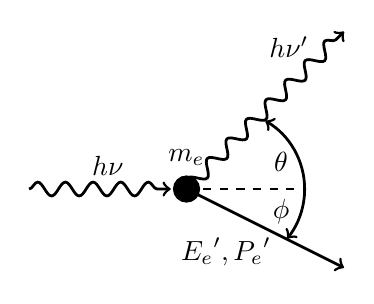
\begin{tikzpicture}
\draw [->, line width=1, snake it](-2,0) -- (-0.2,0);
\node[draw, circle, fill, minimum size=0.2cm] at (0,0) {};
\draw [->, line width=1, snake it](0,0) -- (2,2);
\draw [->, line width=1](0,0) -- (2,-1);
\draw [-, line width=1, dashed](0.0, 0) -- (1.5,0);
\draw[->, line width=1] (1.5,0) arc(0:-39:1);
\draw[->, line width=1] (1.5,0) arc (0:60:1);
\node at (1.2,-0.29) {$\phi$};
\node at (1.2,0.35) {$\theta$};
\node at (0.5,-0.8) {${E_e}', {P_e}'$};
\node at (1.3,1.8) {$h \nu'$};
\node at (-1,0.3) {$h \nu$};
\node at (-0,0.4) {$m_e$};
\end{tikzpicture}
}
\end{minipage}%
%}
%\end{wrapfigure}
\begin{minipage}[r]{0.58\linewidth}
\begin{align*}
& h \nu' = \frac{h \nu}{1 + \frac{h\nu}{m_e c^2} (1 - \cos{\theta})} \\
& \Delta \lambda = \frac{h}{m_e c} (1 - \cos{\theta}) \\
& T_e = h\nu - h\nu' \\
& T_e = h \nu \frac{1-\cos{\theta}}{\frac{m_e c^2}{h \nu} + 1 - \cos{\theta}} \\
& T_\text{max} = \frac{2 h \nu}{2 + m_e c^2 / h \nu} 
\end{align*}
\end{minipage}%
\end{minipage}%
\begin{align*}
\tan{\phi} &= \frac{\sin{\theta}}{(1 + h\nu/m_e c^2)(1-\cos{\theta})} \\
\atan{\frac{\theta}{2}} &= \left(1 + \frac{h \nu}{m_e c^2} \right) \tan{\phi}
\end{align*}
\section{Radioactive Decay}
\begin{align*}
N &- \text{\# Atoms} & \lambda &- \text{Decay Constant} \\
A &- \text{Activity} & SA &- \text{Specific Activity} \\
T_{1 / 2} &- \text{Half life} & M &- \text{Molar Mass}\\
dN &= -\lambda N dt & A &= -\frac{dN}{dt} = \lambda N\\
\frac{N}{N_0} &= \frac{A}{A_0} = e^{-\lambda t} & T_{1 / 2} &= \frac{\ln{2}}{\lambda}
\end{align*} 
\begin{align*}
SA &= \frac{\si{\mole} ~ \lambda}{M} = \frac{\SI{4.17e23}{}}{M~T_{1 / 2}} \\
SA &= \frac{1600}{T (\text{years})} \times \frac{226}{A (\text{Mass \#})} \SI{}{\curie\per\gram}
\end{align*}

\subsection{Decay Chains}
\subsubsection{General Case}
\begin{gather*}
N_n(t) = \prod_{j=1}^{n-1} \lambda_j \sum_{i=1}^n \sum_{j=i}^n 
\left ( \frac{N_i(0)e^{-\lambda_j t}}{\prod_{p=i, p\neq j}^n (\lambda_p-\lambda_j)} \right ) \\
N_n(t) \simeq N \frac{\lambda_j}{\lambda_n} \exp{-\lambda_j t} \quad \lambda_j \ll \lambda_1 \ldots \lambda_n
\end{gather*}

\subsubsection{Decaying Daughter}
\[N_2 = \frac{\lambda_1 N_{1_0}}{\lambda_2 - \lambda_1} \left( e^{-\lambda_1 t} - e^{-\lambda_2 t} \right) \]

\subsubsection{Secular Equilibrium $(T_1 \gg T_2)$}
\begin{align*}
\frac{dN_2}{dt} &= A_1 - \lambda_2 N_2 \\
A_2 &= A_1 \left( 1 - e^{\lambda_2 t} \right) + A_{2_0} e^{-\lambda_2 t}
\end{align*}
If $A_{2_0} = 0,~t \gtrsim 7~T_2$ then $A_1 = A_2$.

\subsubsection{Transient Equilibrium $(T_1 \gtrsim T_2)$}
\[ \lambda_2 N_2 = \frac{\lambda_2 \lambda_1 N_{1_0} e^{-\lambda_1 t}}{\lambda_2 - \lambda_1} = A_2 \frac{\lambda_2 A_1}{\lambda_2 - \lambda_1} \]
\begin{align*}
& \text{Max } A_2 & t &= \frac{1}{\lambda_2 - \lambda_1} \log{\frac{\lambda_2}{\lambda_1}} \\
& \text{Max } A_1 + A_2 & t &= \frac{1}{\lambda_2 - \lambda_1} \log{\frac{\lambda^2_2}{2\lambda_1\lambda_2 - \lambda^2_1}}
\end{align*}

\subsection{Decay Channels}

\subsubsection{$\alpha$ Decay: \textnormal{$\text{P}^A_Z \rightarrow \text{D}^{A-4}_{Z-2} + \text{He}^4_2$}}

Usually heavy elements ($Z \geq 83$). Short range, usually radioactive daughters, harmful if inhaled or ingested. Radium, an $\alpha$ emitter seeks bone
\begin{gather*}
Q_\alpha = \Delta_P - \Delta_D - \Delta_{\text{He}} = E_\alpha + E_{M_N} \\
E_\alpha = \frac{m~Q_\alpha }{m_\alpha + M_N} \quad E_{M_N} = \frac{M_N~Q_\alpha}{m_\alpha + M_N}
\end{gather*}

\subsubsection{$\beta^-$ Decay: \textnormal{$\text{P}^A_Z \rightarrow \text{D}^A_{Z+1} + \beta^0_{-1} + \bar{\nu}^0_0$}}

Pure $\beta^-$ emitters: H\textsuperscript{3}, C\textsuperscript{14}, P\textsuperscript{32}, Sr\textsuperscript{90}, Y\textsuperscript{90} \\
Mixed $\beta^- / \gamma$ emitters: Co\textsuperscript{60}, Cs\textsuperscript{137} \\
Can penetrate skin, internal hazard. \SI{}{\mega\electronvolt} $\beta^-$ can emit bremsstrahlung in heavy-metal shielding, creating $\gamma$ hazard
\begin{gather*}
Q_{\beta^-} = \Delta_P - \Delta_D = E_{\beta^-} + E_{\bar{\nu}} \\
0 \leq E_{\beta^-} \leq Q_{\beta^-} \quad \bar{E}_{\beta^-} \simeq Q_{\beta^-} / 3
\end{gather*}

\subsubsection{$\beta^+$ Decay: \textnormal{$\text{P}^A_Z \rightarrow \text{D}^A_{Z-1} + \beta^0_{+1} + \nu^0_0$}}
Same effect as electron capture. Accompanied by annihilation $\gamma$, $E_\gamma = \SI{0.511}{\mega\electronvolt}$. Competes with EC.
\begin{gather*}
Q_{\beta^+} = \Delta_P - \Delta_D - 2 m_e c^2 \\ 
\Delta_P - \Delta_D > 2 m_e c^2 = \SI{1.022}{\mega\electronvolt}
\end{gather*}

\subsubsection{$\gamma$ Decay: \textnormal{$\text{P}^A_Z \rightarrow \text{D}^{A}_{Z} + \gamma^0_0$}}

$\gamma$ emissions energies create isotope signatures, basis of $\gamma$ spectroscopy. Nuclear excited state lifetimes of $\gamma$ decay typically \SI{10e-10}{\second}, except for much longer lived metastable states. Deeply penetrating, dominates over EC for light nuclei.
\[ Q_\gamma = \Delta_P - \Delta_D \]

\subsubsection{Internal Conversion (IC)}

Alternative to $\gamma$ emission where nuclear excitation energy is transferred to K or L shell electron, ejecting from atom. Usually followed by fast $\gamma$ emission. Dominates for heavy nuclei
\[ \alpha = \frac{N_e}{N_\gamma} \quad E_e = E^* - E_B \]
$\alpha$, IC coefficient for nuclear transition, increases with $Z^3$, decrease with $E^*$.

\subsubsection{Electron Capture (EC): \\ \textnormal{$\text{P}^A_Z + e^0_{-1} \rightarrow \text{D}^{A}_{Z-1} + \nu^0_0$}}

Nucleus captures orbital electron, outgoing neutrino energy $E_\nu = Q_{EC}$. Leaves inner shell vacancy, emitting X-rays and auger electrons of characteristic energies. With electron binding energy $E_B$,
\[ Q_{EC} = \Delta_P - \Delta_D - E_B \quad \Delta_P - \Delta_D > E_B \]

\section{Nuclear Reactions}
\subsection{Mass Excess}
\[ \Delta_\text{Atom} = \text{Z} \times \text{M}_\text{Proton} + (\text{A-Z}) \times \text{M}_\text{Neutron} - \text{M}_\text{Atom}
\]
\subsection{Energy Released}
$ a + b \rightarrow c + d$ or $a(b,c)d$ \\
$Q$, energy released, =
\[Q = [(M_a + M_b) - (M_c + M_d)] c^2\]
$Q > 0$ is exothermic, $Q < 0$ is endothermic

\subsection{Cross Sections}
Reaction Rate $R$, microscopic cross-section $\sigma$
\[ R~[\SI[per-mode=fraction]{}{\number\per\square\centi\metre\per\second}] = \sigma~[\SI[per-mode=fraction]{}{\square\centi\metre}]~ I~[\SI[per-mode=fraction]{}{\number\per\square\centi\metre\per\second}]~ N_A~[\SI[per-mode=fraction]{}{\number\per\square\centi\metre}] \]
\[
R = \Sigma_T I \qquad \Sigma_T = N \sigma_T
\]

Beam $I$, macroscopic cross-section $\Sigma_T$
\begin{align*}
I(x) &= I_0 \exp{-\Sigma_T x} \\
\Sigma_T &= N_X \sigma^X_t + N_Y \sigma^Y_t + N_Z \sigma^Z_t + \ldots = \frac{1}{\lambda}
\end{align*}
$\lambda = $ Mean free path (until 1\textsuperscript{st} interaction)
$\nu~\Sigma_T = [\SI{}{\per\second}]$ Collision Freq., $\nu = $ neutron speed

\subsubsection{Neutron Cross Section Hierarchy}
\resizebox{\linewidth}{!}{%
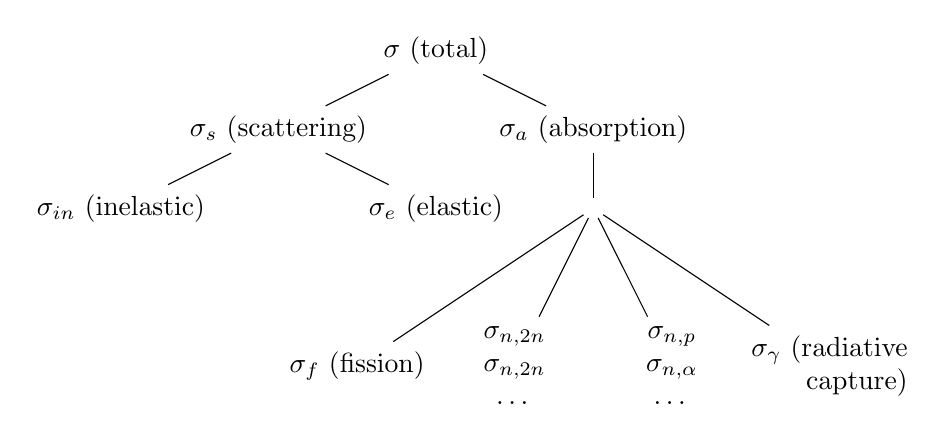
\begin{tikzpicture}
\node (v1) at (0,3) {$\sigma$ (total)};
\node (v2) at (-2,2) {$\sigma_s$ (scattering)};
\node (v3) at (2,2) {$\sigma_a$ (absorption)};
\draw  (v1) edge (v2);
\draw  (v1) edge (v3);
\node (v5) at (0,1) {$\sigma_e$ (elastic)};
\node (v4) at (-4,1) {$\sigma_{in}$ (inelastic)};
\draw  (v2) edge (v4);
\draw  (v2) edge (v5);
\node (v6) at (2,1) {};
\draw  (v3) edge (v6);
\node (v7) at (-1,-1) {$\sigma_f$ (fission)};
\node [align=center] (v8) at (1,-1) {$\sigma_{n,2n}$ \\ $\sigma_{n,2n}$ \\ \ldots};
\node [align=center] (v9) at (3,-1) {$\sigma_{n,p}$ \\ $\sigma_{n,\alpha}$ \\ \ldots};
\node [align=right] (v10) at (5,-1) {$\sigma_\gamma$ (radiative \\ capture)};
\draw  (v6) edge (v7);
\draw  (v6) edge (v8);
\draw  (v6) edge (v9);
\draw  (v6) edge (v10);
\end{tikzpicture}
}

\section{Radiation In Matter}
Single collision, incoming particle ($M$, $E$) can transfer at most $Q_max$ to resting particle $m$
\[ Q_{max} = \frac{2 \gamma^2 m V^2}{1 + 2 \gamma m / M + m^2 / M^2} \simeq \frac{4 m M E}{(M+m)^2} \]
\[ Q_{max} \simeq 2 \gamma^2 m V^2 = 2 \gamma^2 m c^2 \beta^2 \quad \gamma m / M \ll 1 \]
As $E$ increases, $Q_{max} / E \rightarrow 1$ \\

Can define Linear Energy Transfer (LET)
\[
L \equiv \frac{dE}{dl}
\]
$dE$ is energy lost by \textbf{charged} particle due to atomic electron collisions travelling distance $dl$ \\ \\
Related to Lineal Energy
\[
y \equiv \frac{\epsilon}{\bar{l}}
\]
$\epsilon$ is energy imparted to matter in volume, $\bar{l}$ is mean chord length of volume \\

\subsubsection{Stopping Power, $S$}
Avg total linear energy loss rate in matter
\[ S = -\frac{dE}{dx} \]
HCP and $\beta$ particles in matter eject atomic electrons, creating Delta Rays.

\subsubsection{Restricted Stopping Power $S_\Delta$}
Linear rate of energy loss due to collisions where energy transfer does not exceed $\Delta$. Related to Linear Energy Transfer (LET). 
\[
\text{LET}_\Delta = \left( - \frac{dE}{dx} \right)_\Delta \quad S = \text{LET}_\infty = \left( - \frac{dE}{dx} \right)_\infty
\]

\subsubsection{Mass Stopping Power}
\[
\frac{S}{\rho} = - \frac{1}{\rho} \frac{dE}{dx} \left[ \si[per-mode=symbol]{\mega\eV\square\centi\meter\per\gram} \right] \qquad
\rho = \text{density}
\]
For compound of multiple elements
\[
\frac{S}{\rho} = \sum_i \frac{S_i}{\rho_i}
\]

\subsection{Heavy Charged Particles (HCP)}
\subsubsection{Stopping Power}
Bethe Formula for Stopping Power:
\begin{align*}
- \frac{dE}{dx} & = \frac{4 \pi k^2_0 z^2 e^4 n_e}{m_e c^2 \beta^2} \left[ \ln{\frac{2 m c^2 \beta^2}{I (1 - \beta^2)}} - \beta^2 \right] \\
 & = \frac{\SI{5.08e-31}{} z^2 n_e}{\beta^2} \left[ F \left( \beta \right) - \ln{I_\text{eV}}  \right] \si{\mega\eV\per\centi\meter} \\
 F \left( \beta \right) & = \ln{\frac{\SI{1.02e6}{} \beta^2}{1-\beta^2} - \beta^2} \\
z & = \text{atomic number of HCP} \\
n_e & = \text{electrons per unit volume in medium} \\
I & = \text{mean excitation energy of medium} \\
I & \simeq
\begin{array}{lr}
\begin{cases}
\SI{19.0}{\eV}         & Z = 1~(\text{hydrogen}) \\
11.2 + 11.7 Z \si{\eV} & 2 \leq Z \leq 13 \\
52.8 + 8.71 Z \si{\eV} & Z > 13
\end{cases}
\end{array}
\end{align*}
\[
n_e \ln{I} = \sum_i N_i Z_i \ln{I_i}
\]

\subsubsection{Range $R(\beta)~[\si{\gram\per\square\centi\meter}]$}
\begin{align*}
R (\beta) & = \frac{M}{z^2} f(\beta) &  f(\beta) & = \int_0^\beta \frac{g(\beta')}{G(\beta')} d\beta' \\
\frac{R_1 (\beta)}{R_2 (\beta)} & = \frac{z_2^2 M_1}{z_1^2 M_2} & R(\beta) & = \frac{M}{z^2} R_p (\beta)
\end{align*}
Where $R_p (\beta)$ is the proton range in the material

\subsubsection{Slowing Down Time $\tau$}
Time to stop HCP in matter
\[
\tau \sim \frac{\text{T}}{V (-dE / dx)} \qquad \text{K.E. = T, V = velocity}
\]

\subsection{Electrons / Positrons ($\beta^\pm$)}
Can emit through collisional and radiation (bremmstrahlung)
\[
\left( - \frac{dE}{dx} \right)^\pm_\text{tot} = \left( - \frac{dE}{dx} \right)^\pm_\text{col} + \left( - \frac{dE}{dx} \right)^\pm_\text{rad}
\]
\subsubsection{Collisional Stopping Power}
\begin{flalign*}
& \left( - \frac{dE}{dx} \right)^\pm_\text{col} = \\
& \frac{\SI{5.08e-31}{} n_e}{\beta^2} \left[ G^\pm (\beta) - \ln{I_\text{eV}} \right] \si{\mega\eV\per\centi\meter} \\
& G^\pm (\beta) = \ln{(\SI{3.61e5}{} \tau \sqrt{\tau + 2})} + F^\pm (\beta) \\
& F^- (\beta) = \frac{1-\beta^2}{2} \left[ 1 + \frac{\tau^2}{8} - (2 \tau + 1) \ln{2} \right] \\
& F^+ (\beta) = \\
& \ln{2} - \frac{\beta^2}{24} \left[ 23 + \frac{14}{\tau + 2} + \frac{10}{(\tau + 2)^2} + \frac{4}{(\tau + 2)^3}\right]
\end{flalign*}
\subsubsection{Radiative Stopping Power}
\[
\frac{(-dE/dx)_{\text{rad}}^-}{(-dE/dx)_{\text{col}}^-} \simeq \frac{ZE_{e^-}}{800} \quad Z = \text{Material Z}
\]
Radiation Yield $Y$, amount of energy released as bremmstrahlung while slowing down completely
\[
Y \simeq \frac{\SI{6e-4} Z T}{1 + \SI{6e-4}{} Z T}
\]
\subsubsection{Range, $R(T)~[\si{\gram\per\square\centi\meter}]$}
\begin{align*}
& 0.412~T^{1.27 - 0.0954 \ln{T}} & 0.01 \leq T & \leq 2.5~\si{\mega\eV} \\
& 0.530 T - 0.106 & T & > 2.5~\si{\mega\eV}
\end{align*}

\subsubsection{Slowing Down Time $\tau$}
Same as HCP

\subsection{Photons ($\gamma$)}
\section{Dose Quantities}


\subsection{Absorbed Dose}
For mass $dm$ with mean energy imparted $d\bar{\epsilon}$ by ionizing radiation
\[
D \equiv \frac{d\bar{\epsilon}}{dm} \qquad \dot{D} \equiv \frac{dD}{dt}
\]
Measured in Gray
\[
\SI{1}{\gray} = \frac{\SI{1}{\joule}}{\SI{1}{\kilo\gram}} = \SI{100}{\rad} \\
\]
For thin layer with constant stopping power,
\[D = \left( \frac{1}{\rho} \frac{dE}{dx} \right) \Phi \quad \Phi = \text{Flux} \left[ \si[per-mode=symbol]{\number\per\square\centi\meter\per\second} \right] \] 

\subsection{Quality Factor}
Q weights absorbed dose to the biological effectiveness of \textbf{charged} particles producing absorbed dose. Function of LET 

\subsection{Dose Equivalent, $H$}
\[
H \equiv Q D
\]
Used for routine radiation limits, not for acute doses \\
Measured in Sieverts
\[
\SI{1}{\sievert} = \frac{\SI{1}{\joule}}{\SI{1}{\kilo\gram}} = \SI{100}{\rem} \\
\]

\subsection{Equivalent Dose, $H_T$}
\begin{align*}
H_T & \equiv \sum_R w_R D_{T,R} \\
D_{T,R} & \equiv \text{Mean tissue dose of radiation type R} \\
w_R & \equiv \text{Radiation weighting factor}
\end{align*}
Radiation weighting factor relates type of particle or radiation for effectiveness of producing an absorbed dose

\subsubsection{Effective Dose, $E$}
\[
E \equiv \sum_T w_T H_T = \sum_T w_T \sum_R w_R D_{T,R}
\]
$w_T$ is the tissue weighting factor, accounting for relative detriment
\section{Radiation Exposure}
Annual per capita Eff. Dose (2000 UNSCEAR)
\begin{center}
\begin{tabular*}{\linewidth}{@{\extracolsep{\fill}} l l }
\hline
Sources & \makecell{Annual Effective \\ Dose (mSv)} \\
\hline
Background & \\
~Cosmic Rays & 0.4 \\
~Terrestrial $\gamma$ Rays & 0.5 \\
~Inhalation (radon) & 1.2 \\
~Ingestion & 0.3 \\
~Total & 2.4 \\
 & \\
Medical & 0.4 \\
Atmos. Weapon Tests & 0.005 \\
Nuclear Power & 0.0002 \\
\hline
\end{tabular*}
\end{center}
\section{Nuclear Reactors}
\textbf{Light Water Reactor (LWR)} \\
Reactor which uses ordinary water as coolant \\
\textbf{Boiling Water Reactor (BWR)} \\
LWR which allows water to boil in the core. Single loop, steam directly drives generator. Requires powered pumps for circulation and emergency cooling water \\
\textbf{Pressurized Water Reactor (PWR)} \\
LWR where high maintained pressure prevents water boiling. Transfers heat to second water loop which is converted to steam for power \\
\textbf{Canada Deutrium Uranium (CANDU)} \\
$\text{D}_{2}\text{O}$ cooled reactor for better moderation allowing low enriched fuels (nat. uranium). Horizontal fuel bundles, continuous refueling, no outages. \\
\textbf{High Temperature Gas Reactor (HTGR)} \\
High-temperature gas-cooled reactor using pressurized helium. Inherently safe, less fuel \\
\textbf{Liquid Metal Fast Breeder Reactor (LMFBR)} \\
Fast fission, no moderator, typically sodium cooled. Use natural or enriched uranium or plutonium. \\

\subsection{Chain Reactions}
For $\nu$ neutrons released per fission,
\begin{align*}
\eta &= \nu \frac{\sigma_\text{fission}}{\sigma_\text{abs}} \\
\frac{\sigma_\text{fission}}{\sigma_\text{abs}} &= \text{Prob. of Fission per Absorption} \\
\eta > 1 & \quad \text{Chain reaction possible} \\
\eta > 2 & \quad \text{Breeding, creating more fuel, possible}
\end{align*}
Multiplication factor $k$,
\[
k = \frac{\text{\# Neutrons in Generation i}}{\text{\# Neutrons in Generation i+1}}
\]
Can be expressed through the fractional change of neutrons per generation, $\rho$
\[
\rho = (k-1)/k
\]
\begin{align*}
k < 1 & ~~ \rho < 0 & & \enskip \text{Subcritical, reactor shutdown} \\
k = 1 & ~~ \rho = 0 & & \enskip \text{Critical, maintain reactor power} \\
k > 1 & ~~ \rho > 0 & & \enskip \text{Supercritical, reactor startup} 
\end{align*}
With a time $\theta$ between neutron generations, the reactor period $\tau$
\[
\tau = \theta / \ln{k}
\]
Delayed n from fission frag., yield $\beta$, increase $\theta$ \\
Reactor Power increases as
\[
P / P_0 = e^{t \ln{(k)} / \theta}
\]
\begin{align*}
k < 1 + \beta & \qquad \parbox{0.7\linewidth}{Reaction rate controlled by delayed neutrons} \\
k > 1 + \beta & \qquad \parbox{0.7\linewidth}{Prompt super critical, driven by prompt neutrons, uncontrollable}
\end{align*}



\subsection{Six Factor Formula}
\resizebox{\linewidth}{!}{%
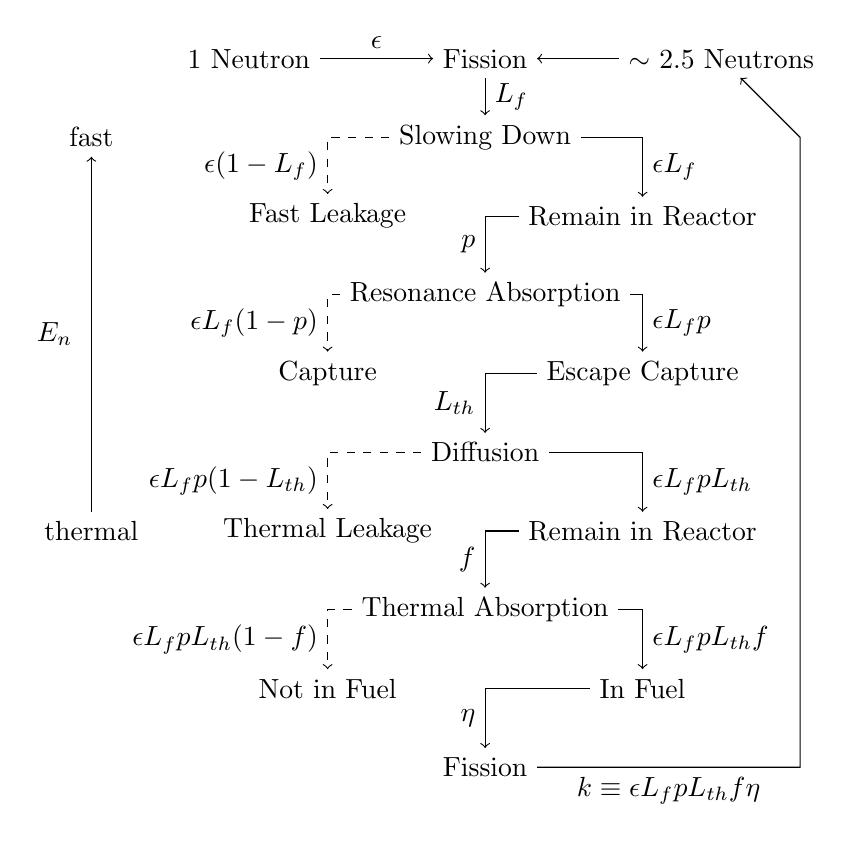
\begin{tikzpicture}
\node (v0) at (-3,0) {1 Neutron};
\node (v1) at (0,0) {Fission};
\draw [->] (v0) edge node[midway, above] {$\epsilon$} (v1);
\node (v3) at (0,-1) {Slowing Down};
\draw [->] (v1) edge node[midway, right] {$L_f$} (v3);
\node (v2) at (-2,-2) {Fast Leakage};
\node (v4) at (2,-2) {Remain in Reactor};
\node (v5) at (0,-3) {Resonance Absorption};
\node (v6) at (-2,-4) {Capture};
\node (v7) at (2,-4) {Escape Capture};
\node (v8) at (0,-5) {Diffusion};
\node (v9) at (-2,-6) {Thermal Leakage};
\node (v10) at (2,-6) {Remain in Reactor};
\node (v11) at (0,-7) {Thermal Absorption};
\node (v12) at (-2,-8) {Not in Fuel};
\node (v13) at (2,-8) {In Fuel};
\node (v14) at (0,-9) {Fission};
\node (v15) at (3,0) {$\sim$ 2.5 Neutrons};
\node (v16) at (-5, -6) {thermal};
\node (v17) at (-5, -1) {fast};
\draw [->, dashed] (v3) -- (-2,-1) -- node[midway, left] {$\epsilon (1-L_f)$} (v2);
\draw [->] (v3) -- (2,-1) -- node[midway, right] {$\epsilon L_f$} (v4);
\draw [->] (v4) -- (0,-2) -- node[midway, left] {$p$} (v5);
\draw [->, dashed] (v5) -- (-2,-3) -- node[midway, left] {$\epsilon L_f (1-p)$} (v6);
\draw [->] (v5) -- (2,-3) -- node[midway, right] {$\epsilon L_f p$} (v7);
\draw [->] (v7) -- (0,-4) -- node[midway, left] {$L_{th}$} (v8);
\draw [->, dashed] (v8) -- (-2,-5) -- node[midway, left] {$\epsilon L_f p (1-L_{th})$} (v9);
\draw [->] (v8) -- (2,-5) -- node[midway, right] {$\epsilon L_f p L_{th}$} (v10);
\draw [->] (v10) -- (0,-6) -- node[midway, left] {$f$} (v11);
\draw [->, dashed] (v11) -- (-2,-7) -- node[midway, left] {$\epsilon L_f p L_{th} (1-f)$} (v12);
\draw [->] (v11) -- (2,-7) -- node[midway, right] {$\epsilon L_f p L_{th} f$} (v13);
\draw [->] (v13) -- (0,-8) -- node[midway, left] {$\eta$} (v14);
\draw [->] (v15) -- (v1);
\draw [->] (v14) -- node[midway, below] {$k \equiv \epsilon L_f p L_{th} f \eta$} (4,-9) -- (4,-1) -- (v15);
\draw [->] (v16) -- (v17) node[midway, left] {$E_n~$};
\end{tikzpicture}
}
\[
k \equiv \epsilon ~ p ~ f ~ \eta ~ L_f ~ L_t
\]
\begin{align*}
\epsilon & \quad \text{fast fission factor} \\
p & \quad \text{resonance escape prob} \\
f & \quad \text{thermal utilization factor} \\
\eta & \quad \text{\# neutrons per abs. in fuel} \\
L_f & \quad \text{fast non-leak prob} \\
L_t & \quad \text{thermal non-leak prob}
\end{align*}
\[
f = \frac{\Sigma_a^\text{fuel}}{\Sigma_a^\text{all mat}} \quad \eta = \frac{\nu \sigma_\text{fiss}^\text{fuel}}{\sigma_\text{abs}^\text{fuel}}
\]

For infinite reactor with no leakage
\[
k_\infty = \epsilon ~ p ~ f ~ \eta
\]

\subsection{Reactor Kinetics}
\[
k = \frac{P(T)}{L(T)} = \frac{\text{Neutron Production Rate}}{\text{Neutron Loss Rate}}
\]
Neutron lifetime $l$ ($\theta$) and reactor period $T$ ($\tau$)
\[
l = \frac{N(T)}{L(T)} \qquad T = \frac{l}{k-1}
\]
\[
N(T) = N_0 e^{t/T}
\]

\subsection{Neutron Diffusion}
\begin{gather*}
-D \nabla^2 \Phi(\vec{r}) + \Sigma_R \Phi(\vec{r}) = S(\Phi(\vec{r})) \\
S(\Phi(\vec{r})) = \nu \Sigma_f \Phi(\vec{r}) \\
D = 1 / 3 ~ \Sigma_{tr} \\
\Sigma_{tr} = \Sigma_T - \mu_0 \Sigma_s \\
L = \sqrt{D / \Sigma_a}
k = \frac{B_m^2}{B_g^2}
\end{gather*}
\section{Misc.}
\subsection{Fission}
${\langle E \rangle}_{\text{fission}} \simeq \SI{200}{\mega\electronvolt}$
\begin{align*}
80\% &= \text{K.E. Fission frag.} & 3\% &= \text{K.E.} \ \text{n}_{\text{fast}} \\
4\% &= \gamma & 4\% &= \beta \ \text{decay frag.} \\
5\% &= \nu & 4\% &= (\text{n},\gamma)
\end{align*}

\rule{0.3\linewidth}{0.25pt}
\scriptsize

Copyright \copyright\ 2015 Aaron Nowack

Adapted from \LaTeXe\ Cheat Sheet \copyright\ by Winston Chang 2014
\href{http://www.stdout.org/~winston/latex/}{http://www.stdout.org/$\sim$winston/latex/}


\end{multicols*}
\end{document}